\section{Introduction}
%introduction结构:
%核心问题:探究狗的声学特点是否会受到特定文化,即其所在环境里主人的语言系统的影响。

%介绍引入:为什么会有这个问题。我们试图去理解狗的语言,那么这个问题的一个key在于狗是否拥有自己后天发展的语言系统。语言的重点落在生物与周遭的环境以及生物的交互上,若能说明狗的语言会受到环境的影响,则可以为后续interpreting它打下基础。

%介绍狗的声学特点,分析其“语言”的性质(其他的特点)
    
%In this work环节
    %as 现在市面上没有特定狗种的数据集,我们构建了一个数据集
    % 提取了若干种音频特征,并且在三种模型上进行了general以及scene-specific的实验
    % 进一步分析实验结果,针对关键的声学特征进行分析,证明狗的声学特点的确会受到特定文化的影响。
    
%our contribution summarized as below:
    %构建了YouDogs数据集,并构建了一个具有拓展性的工程代码
    %在若干种音频特征上完成实验
    %对实验结果进行了分析,确定了xxxx。

%\KZ{Don't forget articles ``the'', ``a'' in your sentences!}

Understanding the language of dogs is an interesting scientific challenge. People have been trying to comprehend what dogs want to express for a number of reasons, such as for better learning about animal biology evolution\cite{pongracz2017modeling}, applying their language to information technology, or just curiosity about dogs' intention when they bark~\cite{pongracz2011children,dogbark_1}. However, this task is challenging not only for the unknown language pattern of dogs, but also the lack of high-quality dataset.
%\MYW{The first sentence should be expanded to a small paragraph indicating why this topic is interesting and challenging}

In this paper, we define the language of dogs as their chief audio communication mode, which is barking. One ubiquitous feature of any natural language is that it does evolve with the interaction with the environment and creatures around it\cite{arnold2018affect}. 

During past studies, prior research has demonstrated that language of dogs indeed reflect their individual state~\cite{pongracz2010barking,larranaga2015comparing}, emotional expression~\cite{thorndike2017animal,hantke2018my,paladini2020bark} and scene understanding~\cite{larranaga2015comparing, molnar2008classification}. However, no one thus far looked into the influence of the interaction between human hosts and dogs on the language of dogs. In our work, we hypothesize that the language of dogs can developed during that interaction. To verify that, we explore the difference of voice of dogs of certain species between two different host language environments~(\figref{fig:intropic}).

%\MYW{2nd paragraph should focus on the previous investigation towards this topic and then lead to a conclusion that no one has looked into the influence of hosts culture/language on pets, then you smoothly transfer to introduce your work}

\begin{figure}[t]
	\centering
	\scalebox{0.32}{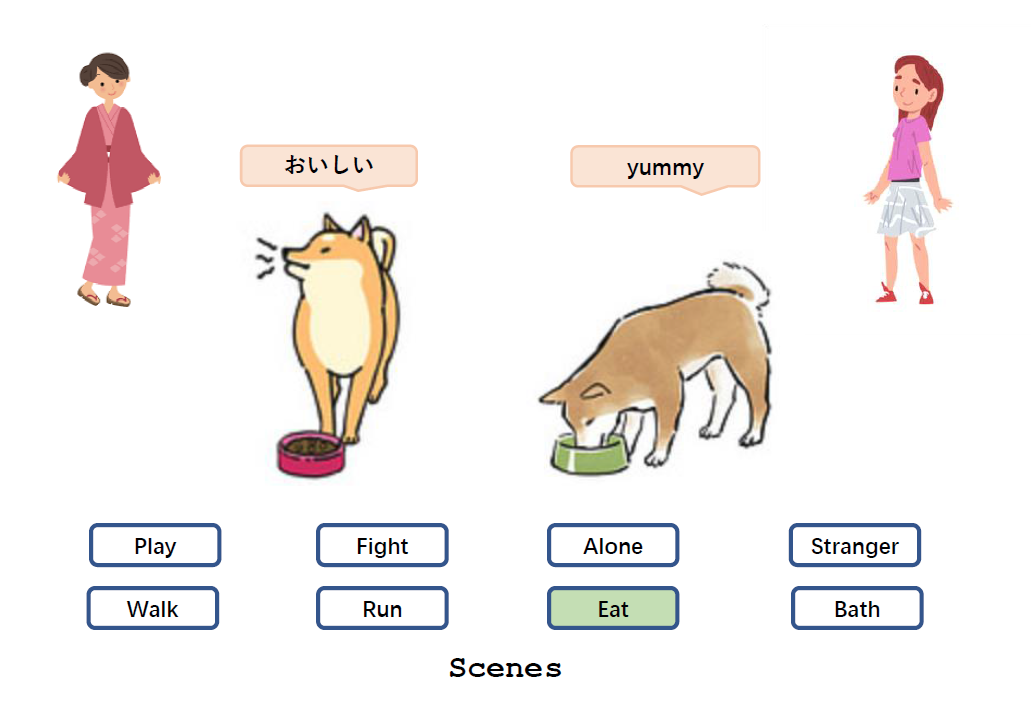
\includegraphics{intropic.png}}
	\caption{During the interaction between dogs and their hosts from different language environments, the barks are possible to diverge.}
	\label{fig:intropic}
\end{figure}


Since there is no existing dataset, we first construct a dataset called ``EJShibaVoice.'' To reduce the influence of noise from certain dog species, we select Shiba Inu dogs to investigate mainly due to the reason that there are a large number of Shiba Inu dogs in Japenese and English language environments. On YouTube, there are a large number of Shiba Inu dogs related videos posted. Thus, We have designed a crawling tool with variable keyword input for YouTube. After gaining the audio set, a sound event detection model is applied to filter the bark clips.

Secondly, we conducted classification experiments to verify that there are certain differences between dog barks from two language environments. To explore the latent factors as much as possible, multiple kinds of features are selected, including mfcc~\cite{davis1980comparison}, mel spectrogram, GeMAPS~\cite{eyben2015geneva}, filterbank~\cite{strang1996wavelets} and PLP~\cite{hermansky1990perceptual}. In the meantime, as barks of dogs are influenced by certain scenes, we try to reduce such kind of noise by doing experiment on specific scene. Differences has been discovered.

Finally, to explain the observed phenomenon, we perform an importance analysis of different factors. Five significant factors which exist in most of the scenes are picked as the prominent factors. The fact that they have substantial correlations with the acoustic characteristics of human voices supports our hypothesis that the host language environment does have a profound influence on dogs' language.

Our contributions are summarized as follows:
%{顺序改一下 重要的放前面 措辞也改一下}
%{加ref到后面的内容}
\begin{itemize}
    \item We define a new task to find out the cultural influence on the language of Shiba Inu dogs, which helps the further research about their language.~(\secref{sec:assumption})
	\item We have found audio difference of dogs from different language environments by testing several kinds of audio features on general and scene-specific classification network to exclude the scene influence.~(\secref{sec:main})
	\item To explain the difference revealed, we have analyzed the prominent features during classification and matched them with human voice characteristics to find a relationship between the voice of dogs and humans.~(\secref{sec:prominentfactor})
	\item We have constructed a Shiba Inu dog barks dataset \textbf{EJShibaVoice} of size 4,463, which contains two different language environments: English and Japanese with eight scenes: play, alone, fight, run, stranger, walk, eat, and bath.~(\secref{sec:assumption})
\end{itemize}
